\documentclass[aps,prl,twocolumn,superscriptaddress,amsmath,nofootinbib,10pt,floatfix]{revtex4-2}
% \usepackage{graphicx}
% \usepackage[normalem]{ulem}
% \usepackage{xcolor}
% %\usepackage{comment}
% \usepackage{textgreek}
% \usepackage[colorlinks, linkcolor=blue, citecolor=blue]{hyperref}
% \usepackage{gensymb}

% \usepackage{amssymb}

% \documentclass[aps,twocolumn,prl,amsmath,nofootinbib,longbibliography,amssymb,superscriptaddress,10pt]{revtex4-2}
% %twocolumn (removed from \documentclass)

\usepackage[english]{babel}
\usepackage{graphicx}
\usepackage{ulem}
\usepackage{soul}
\usepackage{float} %added by Evyatar
%\usepackage{txfonts}
\usepackage[colorlinks, linkcolor=red , citecolor= blue,breaklinks=true]{hyperref}
%\usepackage{breakurl}
\usepackage{bm}
\usepackage{verbatim}
\usepackage{esint}
\usepackage{marginnote}
\usepackage{feynmf}


\Urlmuskip=0mu plus 1mu

\renewcommand{\vec}[1]{\boldsymbol{#1}}
\newcommand{\RNum}[1]{\uppercase\expandafter{\romannumeral #1\relax}}

\def \k {{\vec k}}
\def \p {{\vec p}}
\def \e {\epsilon}
\def \ve {\varepsilon}
\def \r {{\vec r}}
\def \A {\mathrm{A}}
\def \B {\mathrm{B}}
\def \C {\mathrm{C}}
\def \v {{\bf v}}
\def \el {\ell}
\def \s {\vec{s}}
\def \q {{\vec q}}
\def \d{\partial}
\def \Q{{\cal Q}}
\def \l {\ell}
\def \ve {\varepsilon}
\def \dv {\delta\vec{\varphi}}
\def \S {{\cal{S}}}
\def \G {{\cal{G}}}
\def \C {{\cal{C}}}
\def \K {{\vec K}}
\def \x {{\vec x}}
\def \y {{\vec y}}
\def \Y {\mathbb{Y}}
\def \P {\vec{\Phi}}
\def \Ps {\Psi}
\def \Ph{\Phi}
\def \D{\Delta}
\def \t {\theta}
\def \ol{\overline}
\def \n{{\mathbf{n}}}
\def \L{{\cal{L}}}
\def \O {\cal{O}}
\def \beq {\begin{eqnarray}}
\def \eeq {\end{eqnarray}}
\def \tn {\textnormal}
\def \PP {{\cal {P}}}
\def \M{{\cal {M}}}
\def \Z {{\cal {Z}}}
\def \F {{\cal {F}}}
\def \E {{\cal {E}}}
\def \N {{\cal{N}}}
\def \m {{\mathcal}}
\def \kpa {\kappa_\Vert}
\def \kpe {\kappa_\perp}
\def \ol{\overline}
\def \th{\vartheta}
\def \la{\langle}
\def \ra{\rangle}
\def \ua {\uparrow}
\def \da {\downarrow}
\def \tn {\textnormal}
\def \nn {\nonumber}
%\raggedbottom
\newcommand*{\JFM}[1]{\textcolor{cyan}{ JFM: {#1}}}

\begin{document}
\title{$T-$linear resistivity from magneto-elastic scattering: application to PdCrO$_2$}

\author{J.F. Mendez-Valderrama} \thanks{These authors contributed equally to this work}
\affiliation{Department of Physics, Cornell University, Ithaca, New York 14853, USA.}
\author{Evyatar Tulipman} \thanks{These authors contributed equally to this work}
\affiliation{Department of Condensed Matter Physics, Weizmann Institute of Science, Rehovot 76100, Israel}
\author{Elina Zhakina}
\affiliation{Max Planck Institute for Chemical Physics of Solids,
N\"othnitzer Stra\ss e 40, 01187 Dresden, Germany}
\author{Andrew P. Mackenzie}
\affiliation{Max Planck Institute for Chemical Physics of Solids,
N\"othnitzer Stra\ss e 40, 01187 Dresden, Germany}
\affiliation{Scottish Universities Physics Alliance, School of Physics \& Astronomy, University of St. Andrews, St. Andrews KY16 9SS, United Kingdom}
\author{Erez Berg}
\affiliation{Department of Condensed Matter Physics, Weizmann Institute of Science, Rehovot 76100, Israel}
\author{Debanjan Chowdhury}
\affiliation{Department of Physics, Cornell University, Ithaca, New York 14853, USA.}


\date{\today}

\begin{abstract}
An electronic solid with itinerant carriers and localized magnetic moments represents a paradigmatic strongly correlated system. The electrical transport properties associated with the itinerant carriers, as they scatter off these local moments, has been scrutinized across a number of materials. Here we analyze the transport characteristics associated with ultra-clean PdCrO$_2$ --- a quasi two-dimensional material consisting of alternating layers of itinerant Pd-electrons and Mott-insulating CrO$_2$ layers --- which shows a pronounced regime of $T-$linear resistivity over a wide-range of intermediate temperatures. By contrasting these observations to the transport properties in a closely related material PdCoO$_2$, where the CoO$_2$ layers are band-insulators, we can rule out the traditional electron-phonon interactions as being responsible for this interesting regime. We propose a previously ignored electron-magnetoelastic interaction between the Pd-electrons, the Cr local-moments and an out-of-plane phonon as the main scattering mechanism that leads to the significant enhancement of resistivity and a $T-$linear regime in PdCrO$_2$ at temperatures far in excess of the magnetic ordering temperature. We suggest a number of future experiments to confirm this picture in PdCrO$_2$, as well as other layered metallic/Mott-insulating materials.     
\end{abstract}


\maketitle


{\it Introduction.-} Recent years have witnessed a resurgence of interest in the microscopic origin of an electrical resistivity that scales linearly with temperature \cite{chowdhury_sachdev-ye-kitaev_2022,varma_colloquium_2020} and exhibiting a Planckian scattering rate, $\Gamma= Ck_BT/\hbar$, where $C\sim O(1)$ coefficient \cite{bruin_similarity_2013,hartnoll_colloquium_2022,TBG2019,legros_universal_2019,grissonnanche_linear-temperature_2021}. In conventional (simple) metals at room temperature, this phenomenology is readily understood as a consequence of electrons scattering off thermally excited phonons in their equipartition regime \cite{Ziman_2001}. On the other hand, numerous ``correlated" materials belonging to the cuprate  \cite{takagi_systematic_1992,hussey_dichotomy_2011,legros_universal_2019,grissonnanche_linear-temperature_2021}, pnictide \cite{Doiron2009,Shibauchi2014}, ruthenates \cite{Allen1996,klein_anomalous_1996,hussey_normal-state_1998,schneider_low-energy_2014,Rost2011}, rare-earth \cite{stewart_non-fermi-liquid_2001} and moir\'e bilayers \cite{TBG2019,jaoui_quantum_2022} display Planckian scattering down to low temperatures, likely driven by purely electronic interactions and where {\it a priori} it is unclear if phonons play an essential role \cite{bruin_similarity_2013,sds19,das_sarma_strange_2022,hartnoll_planckian_2022}. It is challenging to disentangle the role of electron-electron and electron-phonon interactions on scattering lifetimes. It is quite natural to ask if materials with a nearly identical phonon spectrum and distinct electronic spectra can lead to a distinct temperature dependence of their respective resistivities. 
%%%%%%%%%%%%%%%%%%%%%%%%%%%%%%%%%%%%%%%%%%%%%%%%%%%%%%%%%%%%%%%%%%%%%%%%%
%%%%%%%%%%%%%%%%
\begin{figure}[t]
\centering
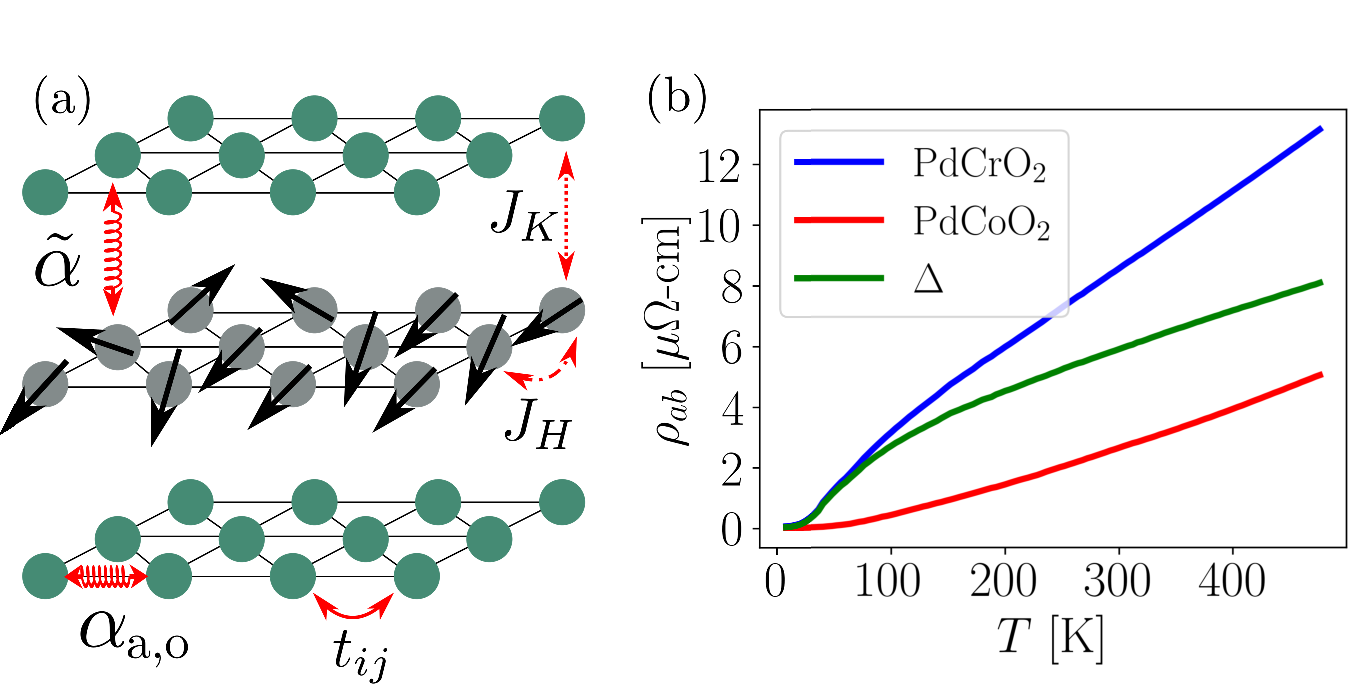
\includegraphics[width=0.5\textwidth]{model_V4.pdf} 
\caption{(a)  The structural motif in PdCrO$_2$, composed of alternating layers of triangular lattices of conducting Pd planes (green) and Mott insulating CrO$_2$ planes (grey). The different coupling constants denoted in the figure are as defined in Eq.~\eqref{total_H}. (b) The in-plane resistivities of PdCrO$_2$ and PdCoO$_2$ taken from Ref.~\cite{Hicks2015} along with their difference $\Delta \rho \equiv \rho_{ab}^{\rm PdCrO_2} -\rho_{ab}^{\rm PdCoO_2} >0$.}
\label{fig:model}
\end{figure}
%%%%%%%%%%%%%%%%

\allowdisplaybreaks{
{\it An experimental puzzle.-} The goal of this letter is to resolve a conundrum inspired by electrical transport measurements in two isostructural quasi two-dimensional compounds with distinct electronic structures: PdCoO$_2$ and PdCrO$_2$. Their structural motif consists of alternately stacked layers of highly conducting Pd and insulating CoO$_2$/CrO$_2$ in a triangular lattice arrangement \cite{eyert_metallic_2008,takatsu_critical_2009,ong_origin_2010,mackenzie_properties_2017,sunko_probing_2020}; see Fig.~\ref{fig:model}(a). The phonon spectra for the two compounds are nearly identical; some of the differences arise from the distinct ionic masses \cite{takatsu_roles_2007,glamazda_collective_2014, mackenzie_properties_2017,sunko_probing_2020}, and recent analysis has also revealed that the unit cell of PdCrO$_2$ is slightly enlarged due to the presence of magnetic moments \cite{Zhakina2023}. On the other hand, their electronic spectra are different since the CrO$_2$ layers are Mott-insulating with the local-moments interacting via antiferromagnetic (AFM) exchange interactions \cite{takatsu_critical_2009,takatsu_magnetic_2014}, while the CoO$_2$ layers are non-magnetic \cite{eyert_metallic_2008,ong_origin_2010,daou_unconventional_2017}. The photoemission spectrum of PdCrO$_2$ contains prominent features, absent in PdCoO$_2$ \cite{noh_anisotropic_2009,noh_direct_2014,sunko_maximal_2017,sunko_probing_2020}, that can be understood from an effective inter-layer Kondo lattice model 
\cite{sunko_probing_2020}. The in-plane resistivities for the two compounds \cite{Hicks2015} are shown in Fig.~\ref{fig:model}(b), respectively. The salient features are as follows: (i) The magnitude of the resistivity for both compounds is small, suggesting that they are ``good" metals with a long mean-free path. (ii) PdCrO$_2$ is considerably more resistive than PdCoO$_2$ over a wide range of temperatures. (iii) PdCrO$_2$ displays a prominent $T-$linear scaling of the resistivity above $T\gtrsim 150$K (far above $T_{\rm N}\approx 37.5$K, the N\'eel temperature for $120^{\circ}-$antiferromagnetism) \cite{takatsu_critical_2009,takatsu_single_2010,takatsu_magnetic_2014,le_magnetic_2018}, and with a slope that is greater than the average slope of $\rho_{ab}(T)$ in PdCoO$_2$ in the same temperature range \cite{Supplementary_material}. 

 The central puzzle that we address in this Letter concerns the microscopic origin of the excess $T-$linear resistivity in PdCrO$_2$ relative to isostructural PdCoO$_2$ ($\Delta \rho \equiv \rho_{ab}^{\rm PdCrO_2} -\rho_{ab}^{\rm PdCoO_2}>0$), going beyond the conventional electron-phonon scattering mechanism, and in a temperature regime where the long-range magnetic order is lost. Given the contrast between PdCrO$_2$ and PdCoO$_2$, it is plausible that the fluctuations of the Cr-local moments play a crucial role on the electronic transport lifetimes even at the relatively high temperatures of interest (i.e. for $T\gtrsim T_N$). However, recent work \cite{mcroberts2022intermediatescale} has demonstrated that electrons scattering off the fluctuations of a ``cooperative" paramagnet \cite{Keren_1994,Moessner_1998L,Moessner_1998B,conlon,Anjana_2017,Mourigal_2019,Shu_2019,Knolle_2022T} can not account for a $T-$linear resistivity; instead the resistivity saturates to a temperature-independent value for $T\gg T_N$. Starting with a microscopic model, we will now demonstrate that the resolution to the conundrum lies in a previously ignored and non-trivial interaction term between the Pd-electrons, the Cr-spins, and phonons, as encoded in an electron-magneto-elastic (EME) coupling. Although specifically motivated by PdCrO$_2$, our theory has relevance beyond this single material. There are a number of exciting new material platforms that have come to the forefront in recent years that consist of stacks of metallic and Mott insulating layers \cite{moirerev,Mak2022,FaiMIT,pasupathyMIT,ajesh,ruhman,moireHF,vavno2021artificial,persky2022magnetic}. In what follows, we develop a general framework to address electrical transport in such layered material platforms, and our conclusions can be used to disentangle the various sources of interaction between electrons, local-moments and phonon degrees of freedom. 
 
 {\it Model.-} Consider a quasi two-dimensional (2D) layered model defined on a triangular lattice, where the electronic and local-moment degrees of freedom reside on alternating layers. The effective 2D Hamiltonian is given by (see \cite{Supplementary_material} for a microscopic derivation of $H_{\rm{EME}}$),
\begin{subequations}
\beq
  H &=& H_{\rm el} + H_{\rm S} + H_{\rm K} + H_{\rm ph} + H_{\rm el-ph} + H_{\rm EME},\nn \label{total_H} \\ \\
H_{\text{el}} & =&\sum_{\boldsymbol{k},\alpha}(\varepsilon_{\boldsymbol{k}} - \mu) p_{\boldsymbol{k}\alpha}^{\dagger}p^{\phantom\dagger}_{\boldsymbol{k}\alpha},\\
H_{\text{S}} & =&J_{\text{H}}\sum_{\left\langle i,j\right\rangle }\boldsymbol{S}_{i}\cdot\boldsymbol{S}_{j},\\
H_{\text{K}} & =&J_{\text{K}}\sum_{i} p^\dagger_{i\alpha} (\boldsymbol{S}_{i}\cdot\boldsymbol{\sigma}_{\alpha\beta}) p^{\phantom\dagger}_{i\beta}, \\
H_{\text{ph}} & =& \sum_{\ell=I_{\rm a},I_{\rm o},O}\sum_{\boldsymbol{q}} \left(\frac{|\pi^{(\ell)}_{\boldsymbol{q}}|^2}{2M} + \frac{M \omega_{\ell,\boldsymbol{q}}^2}{2} |\varphi^{(\ell)}_{\boldsymbol{q}}|^2 \right),\label{phonon_Hamil}\\
H_{\rm{el-ph}} & =& \sum_{i,\sigma} \bigg(\alpha_{\rm a} \nabla \varphi^{(I_{\rm a})}_{i}p_{{i}\sigma}^{\dagger}p^{\phantom\dagger}_{{i}\sigma}+\alpha_{\rm o} \varphi^{(I_{\rm o})}_{i}p_{{i}\sigma}^{\dagger}p^{\phantom\dagger}_{{i}\sigma}\bigg), \\
H_{\text{EME}} & =&\widetilde{\alpha}\sum_{i}\varphi^{(O)}_i p^\dagger_{i\alpha}  (\boldsymbol{S}_{i}\cdot\boldsymbol{\sigma}_{\alpha\beta})p^{\phantom\dagger}_{i\beta}.
\label{EME_Hamiltonian}
\eeq
\end{subequations} 
Here $p^{\dagger}_{\boldsymbol{k}\sigma},~p^{\phantom\dagger}_{\boldsymbol{k}\sigma}$ denote the Pd-electron creation and annihilation operators with momentum $\boldsymbol{k}$ and spin $\sigma=\pm 1/2$. The electronic dispersion is given by $\varepsilon_{\boldsymbol{k}}$ and $\mu$ is the chemical potential; experiments in PdCrO$_2$ indicate the Pd-electronic structure is well captured using first and second-neighbor hoppings and the conduction band, dominantly of Pd character, is very close to half-filling \cite{sunko_probing_2020, Hicks2015}. The local-moments, $\boldsymbol{S}_i$, interact mutually via nearest-neighbor antiferromagnetic Heisenberg exchange ($J_{\rm H}>0$), and with the Pd-electron spin-density via a Kondo exchange ($J_{\rm K}>0$), respectively. The Cr-electrons form $S=\frac{3}{2}$ local-moments \cite{sunko_probing_2020}. Finally, we include three phonon fields, $\varphi^{(\ell)}$ with $\ell=I_{\rm{a}},I_{\rm{o}},~O$, corresponding to in-plane acoustic ($I_{\rm a}$), in-plane optical ($I_{\rm o}$) and out-of-plane ($O$) lattice vibrations, respectively. We set the mass, $M$, to be equal for these modes for simplicity. The in-plane modes $I_{\rm a,o}$ couple to the $p$-electron density with strengths $\alpha_{\rm a,o}$, respectively, while the out-of-plane mode, $O$, couples to the ``inter-layer'' Kondo interaction with EME strength, $\widetilde{\alpha}$. We set the lattice constant $a=1$, unless stated otherwise. Importantly, we include couplings to both in-plane acoustic and optical modes to account for the full $T$-dependence of $\rho_{ab}$ in the absence of magnetism (i.e. in PdCoO$_2$) \cite{takatsu_roles_2007}. Henceforth, we neglect the weak momentum dependence and the form-factors associated with the different interaction terms in the quasi two-dimensional setting to simplify our discussion \cite{sunko_probing_2020}. We will restore these additional complexities when considering out-of-plane transport for reasons to be made clear below.
}

Let us begin by considering the simpler case where the optical modes are Einstein-phonons, with ${\omega}_{I_{\rm o},\boldsymbol{q}} = \omega_0$ and $\omega_{O,\boldsymbol{q}} = \widetilde{\omega}_0$, while for the acoustic mode ${\omega}_{I_{\rm a},\boldsymbol{q}} = cq$, with a corresponding Debye frequency $\omega_D$. The experimental %``intermediate'' 
regime of interest  corresponds to $\{\widetilde{\omega}_0,J_{\rm{H}}\}\lesssim T\ll\ve_F$, where $\ve_F$ is the Fermi energy for the Pd-electrons. Moreover, we shall consider the limit where $ J_{\rm{H}} \gg \{\widetilde{\alpha}\sqrt{\hbar/M\widetilde{\omega}_0},~J_{\rm{K}}\}$ and thereby ignore the feedback of both electrons and phonons on the properties of the local-moments. In recent work \cite{mcroberts2022intermediatescale}, some of us analyzed the properties of a subset of the terms, ($H_{\tn{el}}+H_{\tn{S}}+H_{\tn{K}}$), in Eq.~\eqref{total_H} at leading order in a small $J_{\rm{K}}$ by approximating the local-moments as $O(3)$ vectors, but capturing their complex precessional dynamics using the Landau-Lifshitz equations \cite{Keren_1994,Moessner_1998L,Moessner_1998B,conlon,Anjana_2017,Mourigal_2019,Shu_2019,Knolle_2022T}. While this leads to an interesting frequency dependence and momentum-dependent crossovers in the electronic self-energy, the temperature dependence can be understood entirely based on a high-temperature expansion with uncorrelated local-moments. The present manuscript will treat the local-moments on the same footing, but include the additional interaction effects due to ($H_{\rm{ph}}+H_{\rm{el-ph}}+H_{\rm{EME}}$).

{\it Results for intermediate-scale transport.-} We will analyze electrical transport for the model defined above within the framework of traditional Landau-Boltzmann paradigm \cite{Ziman_2001}. This is justified based on the magnitude of the resistivity being much smaller than the characteristic scale of $ha_B/e^2$ ($a_B\equiv$Bohr radius) and $k_F \ell_{\rm mfp} \gg 1$ over the entire temperature range of interest ($\ell_{\rm mfp}$ being the mean free path) \cite{Hicks2015}. Moreover, there is direct experimental evidence for the value of the dimensionless Kondo-coupling being small, based on recent photoemission experiments \cite{sunko_probing_2020}. 

Considering the full $H$, we have multiple sources of scattering for the electrons. Within Boltzmann theory, the total transport scattering rate satisfies Matthiessen's rule \cite{Ziman_2001}: 
\begin{eqnarray}
\frac{1}{\tau_{\rm tr}} = \frac{1}{\tau_{\rm{el-ph}}} + \frac{1}{\tau_{\rm K}} + \frac{1}{\tau_{\rm EME}},
\label{tr_time}
\end{eqnarray}
and the in-plane resistivity is given by $\rho_{ab} = m/(ne^2 \tau_{\rm tr})$, where $m$ is the effective mass and $n$ is the electron density \cite{Supplementary_material}. Experiments with controlled amounts of irradiation shift the overall resistivity curves by a constant (and relatedly, the residual resistivity), without affecting the slope in the $T-$linear regime \cite{Zhakina2023}.  We start by describing the electron-phonon contribution, $1/\tau_{\rm{el-ph}}\equiv 1/\tau_{\rm{el-ph},a}+1/\tau_{\rm{el-ph},o}$.  
Previous works have obtained $1/\tau_{\rm{el-ph}}$ for PdCoO$_2$, and highlighted the importance of a high-frequency optical mode (which is not entirely in the equipartition regime at $T\lesssim \omega_0$) for the observed superlinear-scaling of $\rho_{ab}(T)$ \cite{takatsu_roles_2007,Hicks_mobility_2012}. We have fully reproduced these results for PdCoO$_2$ based on the same procedure \cite{Supplementary_material} within our 2D  model of the Fermi surface; see Fig.~\ref{fig:main}. In PdCrO$_2$, the scattering of electrons off the local-moments due to the bare Kondo interaction, $1/\tau_{\rm K}$, can lead to a sub-linear $T$-dependent contribution to $\rho_{ab}$ at temperatures $T \gtrsim J_{\rm H}$, before saturating to the $T$-independent value \cite{mcroberts2022intermediatescale} (see $\rho_{\rm K}=m/(ne^2 \tau_{\rm K})$ in the inset of Fig.~\ref{fig:main}).


We now turn to the important role of the EME term in PdCrO$_2$. For $\widetilde{\omega}_0\gtrsim J_{\rm{H}}$  we find that $\tau_{{\rm EME}}^{-1}$ follows closely the temperature dependence of the scattering rate of electrons interacting with an optical mode of frequency $\widetilde{\omega}_0$ with a modified dimensionless coupling, 
 \beq
\lambda_{\rm EME} = \frac{\nu_0 \widetilde{\alpha}^2}{{M}\widetilde{\omega}_0^2}S(S+1).
\label{lambdaeph}
\eeq
Here, $\nu_0$ is the electronic density of states at the Fermi level, and scattering off the (spin$-S$) local-moment fluctuations via the EME interaction leads to the additional factor of $[S(S+1)]$ \cite{Supplementary_material}. Ignoring the constant offset, $1/\tau_{\rm K}$ at $T\gg J_{\rm{H}}$, we find that
\begin{equation}
    \frac{1}{\tau_{\rm tr}} \approx 2\pi\left(\lambda_{\rm{el-ph, a}} +\lambda_{\rm{el-ph, o}} + \lambda_{\rm EME}\right) T,\quad T\gtrsim \omega_0,
    \label{slope_w_EME}
\end{equation}
where the dimensionless coefficients are given by,
\beq
\lambda_{\rm{el-ph,o}} = \frac{\nu_0\alpha^2_{\rm{o}}}{M\omega_0^2},~~\lambda_{\rm{el-ph,a}} = \frac{\nu_0\alpha^2_{\rm{a}}}{Mc^2}.
\label{lambdaeph}
\eeq
Consequently, at the highest temperatures, the effect of the EME term considered in this work is to enhance the slope ($A$) of a $T-$linear resistivity, $\rho_{ab}-\rho_0=AT$. This constitutes our first important result. 

Importantly, note that even if the bare EME coupling is weak relative to the electron-acoustic phonon coupling (i.e. $\widetilde{\alpha}/ \alpha_{\rm{a}} \ll 1$), the dimensionless coupling $\lambda_{\rm EME}$ is not necessarily small compared to $\lambda_{\rm{el-ph,a}}$. Furthermore, if the out-of-plane phonon %were to be considerably 
is soft ($\widetilde{\omega}_0 / \omega_D \ll \widetilde{\alpha}/\alpha_{\rm{a}} $), the presence of the EME interaction can dramatically reduce the onset of $T$--linear resistivity to $\mathcal O(\widetilde{\omega}_0)$. 


Assembling all of the above ingredients, we can now reproduce the resistivity in PdCrO$_2$, including the effect of the EME term; see Fig.~\ref{fig:main}. Note that the scattering rates due to the electron-phonon interaction in PdCoO$_2$ \cite{roles_highfreq_pdcoo2_takatsu_2007, Hicks_mobility_2012} and Kondo coupling in PdCrO$_2$ \cite{sunko_probing_2020} are fixed by previous experiments, which leaves two independent parameters in our theory --- $\lambda_{\rm EME}$ and $\widetilde{\omega}_0$ ($J_{\rm{H}}$ is also fixed \cite{sunko_probing_2020}). We determine these parameters by fitting the excess resistivity $\Delta\rho$ in Fig.~\ref{fig:model}(b) to the analytical form of $\tau_{{\rm EME}}^{-1}$ \cite{Supplementary_material}. The values obtained by this procedure are consistent with the characteristic out-of-plane lattice vibration frequency being naturally softer than the in-plane one,  $\omega_0\gtrsim\widetilde{\omega}_0\gtrsim J_{\rm H}$; however, we note that our theory extends beyond this regime. The resulting contribution to the resistivity, $\rho_{\rm EME}$, is shown in the inset of Fig.~\ref{fig:main}. Overall, the prominent $T$--linear resistivity at intermediate $T$ stems from (i) the EME scattering rate; and (ii) the combined sub- and super-linear contributions of $\rho_{\rm K}$ and $\rho_{\rm{el-ph}}$, respectively
 \cite{Supplementary_material}. 
 

%%%%%%%%%%%%%%%%%%%%%%%%%%%%%%%%%%%%%%%%%%%%%%%%%%%%%%%%%%%%%%%%%%%%%%%%%
%%%%%%%%%%%%%%%%
\begin{figure}[t]
\centering
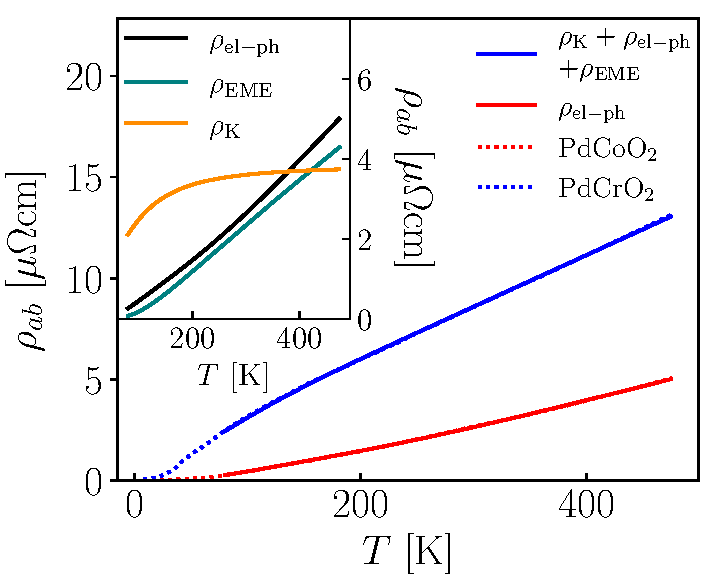
\includegraphics[width=0.45\textwidth]{in-plane.pdf} 
\caption{Comparison of $T-$dependence of in-plane resistivity between experiments \cite{Hicks2015} (dotted lines) and theoretical model in Eq.~\eqref{total_H} (solid lines). The only free parameters in the fits are the phonon frequencies and bare el-ph and EME couplings. All other parameters are fixed; see \cite{sunko_probing_2020,Supplementary_material}. For the phonon data, we have used $\omega_D = 29$meV, $\omega_0 = 120$meV, $\widetilde{\omega}_0 = 40$meV, $\lambda_{\rm{el-ph, a}} = 0.04$, $\lambda_{\rm{el-ph, o}} = 0.02$, $\lambda_{\rm EME} = 0.05$ and $S=3/2$.}
\label{fig:main}
\end{figure}
%%%%%%%%%%%%%%%%


{\it Role of acoustic phonons.-} Our discussion thus far has focused on the simplified limit of an EME coupling to optical phonons. Let us now analyze the effects of an EME coupling to an acoustic phonon. For $H_{\text{ph}}$ in Eq.~\ref{phonon_Hamil}, this amounts to replacing $\widetilde{\omega}_0^2\left(\widetilde{\varphi}^{(O)}_{\vec{q}}\right)^{2}\rightarrow \widetilde{\omega}^2_{\boldsymbol{q}}\left(\widetilde{\varphi}^{(O)}_{\vec{q}}\right)^{2}$, where $\widetilde{\omega}_{\boldsymbol{q}}=\widetilde{c}q$ in the limit of small $q$. Similarly, for $H_{\text{EME}}$ in Eq.~\ref{EME_Hamiltonian}, this amounts to replacing $\varphi^{(O)}_i \to \nabla\varphi^{(O)}_i$. Note that, in practice, the out-of-plane vibrations that couple the layers are at a finite wavevector, namely, 
$\omega_{\boldsymbol{q}} \approx \sqrt{\widetilde{c}^2q_x^2+\widetilde{c}^2q_y^2+ \widetilde{c}_z^2q_{z,0}^2}$ in the limit where $\widetilde{c}_z q_{z,0}\ll T$.  
It is worth noting that unlike the conventional electron-phonon interaction, where scattering is mainly small-angle up to the BG temperature, the EME term induces large-angle scattering even at low-$T$ due to large momentum transfer to the local-moments, which serve as a ``bath". If the spin structure-factor exhibits non-trivial correlations in the Brillouin-zone (i.e. the spin-correlation length is finite with remnants of Bragg-like peaks), the intermediate-scale transport behavior is controlled by the Pd-electron Fermi-surface geometry. However, when the spin-correlation length is short, $1/\tau_{\rm EME}$ shows two distinct regimes~\cite{Supplementary_material}. For $T \gtrsim \widetilde{T}_{\rm BG}\equiv 2\widetilde{c}k_F$, the Bloch-Gr\"uneisen temperature, the result reduces to the case of optical phonons, $1/\tau_{\rm EME}=2\pi \lambda_{\rm EME}T$ with $\lambda_{\rm EME} = \frac{\nu_0 \widetilde{\alpha}^2}{M\widetilde{c}^2}S(S+1)$. On the other hand, for $J_{\rm H} \lesssim T \lesssim \widetilde{T}_{\rm BG}$, we encounter an unexpected $1/\tau_{\rm EME}=2\pi \lambda_{\rm EME}T^2/\widetilde{T}_{\rm BG}$, instead of the usual $\sim T^4$ regime in two-dimensions for the phase-space reasons introduced above. Interestingly, this is an example of a $T^2$ ``quasielastic" scattering due to the EME term (instead of the usual $T^2$ due to umklapp scattering). 


\textit{Effect of $c$-axis strain on in-plane transport.-} Given that the proposed EME interaction in PdCrO$_2$ originates from fluctuations of the (inter-layer) Kondo coupling, applying $c$-axis pressure is expected to enhance the slope of the $T$--linear resistivity for the following reason. The bare EME coupling is controlled in part by the Kondo-scale, $\widetilde{\alpha}\propto t_{cp}^2/U$ where $t_{cp}$ is the inter-plane hybridization between the Pd and Cr-electrons and $U$ is the on-site Coulomb repulsion for Cr-electrons \cite{sunko_probing_2020,Supplementary_material}. Upon applying $c$-axis strain, the inter-layer distance reduces, thereby increasing $t_{cp}$, which is exponentially sensitive to the deformation; the stiffening of the out-of-plane phonons is at best algebraic. Therefore, the dimensionless EME coupling, $\lambda_{\rm EME}\propto t^4_{cp}/(U\widetilde{\omega}_0)^2$ is expected to show a significant increase, along with an enhancement of the Kondo coupling which affects the constant shift in the resistivity at high $T$. The predicted form of the in-plane transport is depicted in the inset of Fig.~\ref{fig:predictions}(b) for a range of $c-$axis strain ($\varepsilon_{zz}$) for bare microscopic parameters as chosen in Fig.~\ref{fig:main}. 


\textit{Out-of-plane transport.-} The electrical resistivity along the $c$-axis provides a direct window into the inter-layer nature of the magnetic interactions, which we have absorbed so far in the effective 2D model. We consider the leading contributions to the $c$-axis conductivity within linear-response theory, which is given by 
\begin{eqnarray}
\sigma_c = \sigma_{\rm coh} + \sigma_{\rm K} + \sigma_{\rm EME},
\label{c_axis_cond_terms}
\end{eqnarray}
where $\sigma_{\rm coh}$ arises from the ``coherent'' channel due to inter-layer $p$ to $p$ hoppings ($t_{pp}$), and $\sigma_{\rm K}$, $\sigma_{\rm EME}$ represent the ``incoherent'' channels due to inter-layer spin-assisted and spin-phonon-assisted contributions, respectively \cite{Supplementary_material}. For simplicity, we ignore the contribution due to an interlayer ``incoherent'' phonon-assisted hopping not involving the local moments; such a term does not affect our results at a qualitative level. The leading-order Feynman diagrams corresponding to each of these contributions  are depicted in Fig.~\ref{fig:predictions}(a). We have $\sigma_{\rm coh} = e^2 (n/m)_c \tau_{\rm tr}$, where $(n/m)_c$ is related to the $c$-axis dispersion and $\tau_{\rm tr}$ is given by Eq.~\eqref{tr_time}; the detailed expressions for the incoherent channels appear in \cite{Supplementary_material}. 


The coherent channel dominates $\sigma_c$ up to temperatures $T\lesssim T_* \sim 10^3~$K (determined by the condition $\sigma_{\rm coh}(T_*) \approx \sigma_{\rm EME}(T_*)$ \cite{Supplementary_material}), such that, in this $T$-regime, $\sigma_c$ and $\sigma_{ab}$ follow the same $T$-scaling as they share the same transport lifetime. The contribution of the incoherent channels becomes significant at temperatures $T\gtrsim T_*$, where, due to the weak $c$-axis dispersion, their temperature dependence is determined by the $T$-scaling of the current vertices, rather than the transport lifetime. In particular, for $T\gtrsim \omega_D,\widetilde{\omega}_0$, while $\sigma_{\rm coh} \sim 1/T$ as in the in-plane case, $\sigma_{\rm K}$ is independent of $T$ and $\sigma_{\rm EME}\propto T$. As a result, the $c$-axis resistivity becomes sublinear at sufficiently high temperatures, as depicted in Fig.~\ref{fig:predictions}(b).


The interplay between the different conduction mechanisms has signatures in the behavior under c-axis pressure. The in-plane conductivity is expected to decrease with c-axis compression, since the EME scattering is enhanced (because it is proportional to the inter-plane hopping strength.)
In contrast, the coherent part of the $c-$axis conductivity increases, as a result of the enhanced inter-layer hopping~\cite{Supplementary_material}. Interestingly, this increase in $\sigma_{\rm coh}$ is associated solely with the el--ph scattering term. The contributions to $\sigma_{\rm coh}$ from the Kondo and EME terms are proportional to $t_{pp}^2/t_{cp}^4$~\cite{Supplementary_material}; assuming that $t_{pp}\propto t_{cp}^2$,  
the ratio $t_{pp}^2/t_{cp}^4$ is unchanged by c-axis strain. Similarly, the incoherent parts of the conductivity increase with compression. However, they do so slightly in excess of $\sigma_{\rm coh}$ which in turn reduces the crossover scale $T_*$, as manifested by the increase in curvature at intermediate temperatures with increasing compression; see Fig.~\ref{fig:predictions}(b) \cite{Supplementary_material}.


\begin{figure}[t]
\centering
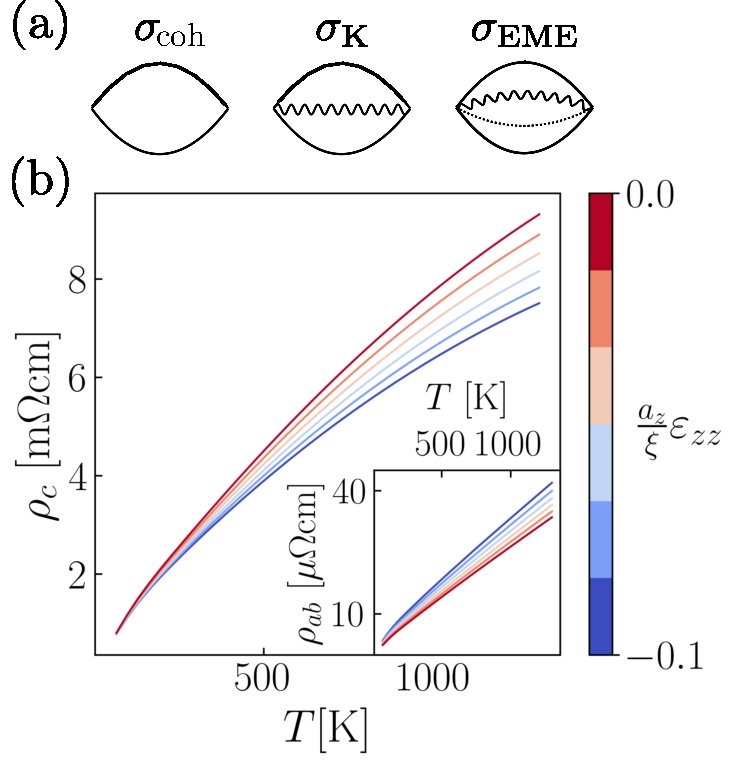
\includegraphics[width=0.45\textwidth]{predictions_v5.pdf} 
\caption{(a) The Feynman diagrams contributing at leading-order to the $c-$axis conductivity, $\sigma_c$ (see Eq.~\eqref{c_axis_cond_terms}), where solid, wiggly and dashed lines denote electrons, spins and phonons, respectively. (b) $c$-axis resistivity as a function of $T$ for different (compressive) $c$-axis strain $\varepsilon_{zz}$ (in units of $\xi/a_z$, where $\xi$ is the characteristic decay length of the hopping integral and $a_z$ is the $\hat{z}$ lattice constant). Inset: in-plane resistivity as a function of $T$ under $c$-axis strain $\varepsilon_{zz}$. 
}
\label{fig:predictions}
\end{figure}
 


{\it Discussion.-} Our conjectured magneto-elastic mechanism for  the enhanced $T-$linear resistivity in PdCrO$_2$ relies on quasi-elastic scattering, where the phonons are in the equipartition regime. There is experimental evidence for the Lorenz ratio satisfying the Wiedemann-Franz law in the $T-$linear regime \cite{Zhakina2023}, which is consistent with our mechanism. Interestingly, the extracted transport scattering rate in the same regime of $T-$linear resistivity is Planckian with $C\approx 0.9$ \cite{Zhakina2023}. Within our model and in the quasi-elastic regime, this is not indicative of any fundamental principle, such as a bound associated with an inelastic scattering rate. It is, however, far from obvious why the scattering rate turns out to be Planckian. 

A natural future direction is to study the effects of the EME term at low temperature.  In particular, the magneto-elastic coupling might be evident in the electronic spectral function. Signatures of phonon drag observed in PdCoO$_2$ \cite{Hicks_mobility_2012} are expected to be suppressed in PdCrO$_2$ due to EME-induced large-angle scattering of phonons off magnetic moments \cite{takatsu_critical_2009}. Pronounced magnetic correlations may also lead to a generalized Kohn anomaly \cite{Kohn_anomaly} associated with phonon softening at the AFM wavevectors. A detailed understanding of the low-temperature properties of this interesting system remains an open problem.

{\it Acknowledgements-} JFMV and DC acknowledge the hospitality of the Weizmann Institute of Science, where this work was completed. JFMV and DC thank A. McRoberts and R. Moessner for an earlier related collaboration \cite{mcroberts2022intermediatescale} and insightful discussions. DC thanks P. Coleman, J. Ruhman, and T. Senthil for useful discussions. DC and EB acknowledge the support provided by the Aspen Center for Physics where this collaboration was initiated, which is supported by National Science Foundation grant PHY-1607611. Research in Dresden benefits from the environment provided by the DFG Cluster of Excellence ct.qmat (EXC 2147, project ID 390858940).


\bibliography{refs.bib}


\end{document}